\documentclass[12pt, fullpage,letterpaper]{article}

% I copied older latex files that include packages we may need but idk,
% I'm not too knowledgeable about all things Latex
\usepackage[margin=1in]{geometry}
\usepackage{url}
\usepackage{amsmath}
\usepackage{amssymb}
\usepackage{amsthm}
\usepackage{xspace}
\usepackage{graphicx}
\usepackage{hyperref}
\usepackage{listings}
\usepackage{bm}
\usepackage{cite}
\usepackage{subfigure}
\usepackage{cite}

\theoremstyle{definition}
\newtheorem{definition}{Definition}[section]

\graphicspath{{./}}
\title{Final Report}
\author{Tyler Adams: u0761872 \\Corbin Baldwin: u0292800}

\begin{document}
	\maketitle 
	\hrule 
	\vskip 0.5cm
%	\section{Paper Rubric}
%	\begin{enumerate}
%		\item Team Members:  the names and UID of your team members.
%		\item Introduction:  Motivation  and  a  brief  project  description.   What  is  the  main  objective  of  your project?  What is an overview of your strategy to achieve your objective?
%		\item Technical Contributions:  What are the technical contributions of your proposed work?
%		\item Data:  What are the type(s) of data your project will be dealing with?  How do you plan to gethold of such data sets?  What kind of insights are you planning to obtain from your data?
%		\item Background and Related Work:  technical background, together with related work.  What are thestate-of-the-art techniques in dealing with the data of your interest?  What are the differences andsimilarities between your work and the state-of-the-art?
%		\item Methods:   What  methods  have  you  used/developed?   What  are  your  strategies  in  tackling  the proposed problem?
%		\item Results and Insights:  What are the results of your proposed project?  What are the key insights?
%		\item Evaluation:  What metrics do you use to evaluate how successful your project is?  What are thetake home messages based on your evaluation?
%		\item Deliverables:  What are your deliverables?  (e.g.  source code,  video demo,  etc.)  What software(and possibly hardware) do you use?  Or in the case you are working on software extensions, whatis the baseline software you work with?
%		\item Conclusions and Dicussions:  answer specific questions below using 1-2 sentences:
%		\begin{itemize}
%			\item What is an overview of your project?
%			\item What are your project objectives?
%			\item What questions does your project address?
%			\item What are the key insights based on your results?
%			\item What are future directions?
%		\end{itemize}
%	\end{enumerate}	
	
	\section*{\normalfont Introduction}
	% Motivation and a brief project description.
	Rayleigh-Taylor instability (RTI) forms at the surface of contact between two fluids, one of which is denser and accelerates toward the other. Formations in RTI are not symmetric between the denser and lighter fluids, and the features of both sides serve to characterize the RTI. However, these features quickly rise in complexity, and it is unrealistic to simulate them beyond a given time threshold. In our project we used machine-learning to construct a classifier that accurately predicts the mixing-specie using topological data analysis (TDA) and other methods learned throughout the course. To do so, we compared two different data structures on which we will train various classifiers. The first uses persistence diagrams constructed using persistent homology on the mixing boundary. The second is constructed on the mixing boundary using what we later define as \emph{critical diagrams}. This path is inspired directly by the material we have learned throughout the course. We will compare the various classifiers and their results using a collection of resources and software, some of which was developed for the second course project.
	
	\section*{\normalfont Technical Contributions}
	
	
	\section*{\normalfont Data}
	The data we used was simulated using the Palabos library, located at \url{http://www.palabos.org/}. This library specializes in modeling fluid dynamics. A \emph{mixing class} is an ordered pair $(\rho_1, \rho_0)$ of densities of fluids whereby $\rho_1$ is the density of the heavier top fluid and $\rho_0$ is the density of the lighter bottom fluid. Using the above mentioned software, we chose four mixing classes, 
	$$
		(1.0, 0.0), \ \ (0.8, 0.0), \ \ (1.0, 0.2), \ \ (0.8, 0.2)
	$$
	and for each mixing class we ran 10 simulations. Each simulation had a different randomly generated initial condition leading to different mixing behavior. Both mixing classes $(1.0, 0.0), (0.8, 0.0)$ had 51 images generated during the simulation. The mixing class $(1.0, 0.2)$ had 71 images per simulation and the mixing class $(0.8, 0.2)$ had 67 images per simulation. These images, in \texttt{.gif} format, were the source of our data for the entire project. 
	
	We were unable to use more mixing classes because of the amount of time it takes to run the software and extract boundaries as well as the fact that we were unable to develop robust boundary extraction software for some of the more wild images generated for other mixing specie. Additionally, the densities above are purely numeric, and do not translate directly to real units. No fluid has a density of 0.0. However the software mentioned above was configured to accept ``density'' values in the interval $[0.0, 1.0]$, so we were restricted to this range. Thus the fluid densities do not represent actual existing fluids. % would break whenever we used density values outside the interval $[0.0, 1.0]$
	
	\section*{\normalfont Background and Related Work}
	The inspiration for the project largely came from \cite{paper}. In the paper, the authors simulate RTI and keep track of the bubble evolution using Morse-Smale Complexes. Since we are using two-dimensional images, we believe Morse-Smale complexes are either poorly defined or irrelevant, so we did not directly use their approach. However, we modified it to something that was more applicable to two dimensional RTIs. In tracking bubble evolution to display a merge-split tree, the authors kept track of the critical point locations (maximum critical points, not minimum critical points) by using the Euclidean distance between critical points in successive time steps of the simulation. Given some threshold (Euclidean radius), it seemed that they treated two critical points in two successive iterations as equivalent if they were within this threshold. This was the inspiration for our method of attack as described in the section below. 
	
	We are not aware of any work that tries to classify mixing specie using a machine learning approach. Because of this, we are unable to compare our approach with a state-of-the-art baseline. In lieu of this, because our approach is almost algorithmically-identical to the use of peristent homology in classifying images with which this course gave us much experience, we chose that as our baseline of comparison.
	
	\section*{\normalfont Methods}
	\subsection*{\normalfont Boundary Extraction} Given the images, we needed a method to sample points from the isosurface, or boundary between fluids. For reasons that will become apparant in the \emph{Critical Diagrams} section, we needed to minimize noise around the isosurface, so as to prevent unmeaningful local minima and maxima. To highlight the isosurface, each image was subtracted from a blurred copy of itself. This yielded higher intensity pixels near edges, where the original image had sharp color changes. This new image will be referred to as the \emph{difference image}. We found that we could sharpen the edges more, leading to a more crisp isosurface in the difference image, if we merged the green and red channels of the original before rendering the difference image.
	
	To sample points from the isosurface, a probabilistic approach, where pixels of high intensity in the difference image were more likely to be sampled, turned out to be too noisy. Instead, we designed an algorithm that would follow the isosurface until it returned to its place, selecting points at regular intervals. To do this, we first needed to find a starting point on the isosurface. We did this by choosing the maximum value pixel in a vertical line of the difference image. Then, we would fix a radius, $r$, between points, and choose another point at a distance of $r$ from the first, which had the maximum value. This process would continue iteratively until the algorithm reached the first chosen point.
	
	After each point was chosen, its neighbors were set to black in the difference image, preventing the path from backtracking. Though this algorithm often produced promising results, it would occasionally lose the path of the isosurface and ``wander'' around the image in irregular patterns. To correct this, we reviewed each point set, painted onto the difference image, to ensure that it properly captured the isosurface. When it failed, we would change the configurations slightly (e.g. radius between points, initial vertical line, and blur factor, which determined the intensity of blur used to render the difference image), until the points lied on the isosurface.
	
	Using this method, we managed to sample the isosurfaces with little, if any noise.
	
	\subsection*{\normalfont Persistent Homology}
	For the baseline, we chose the latest images in each simulation for each class as the choice object with which to calculate persistent homology. For example, if we let a simulation run 6000 iterations, we chose the image generated at time 6000 as a representative of this simulation. With this image, we extracted the boundary and computed 0 and 1-dimensional persistent homology and their corresponding persistence diagrams using Ripser. Using these persistence diagrams, we trained classifiers learned throughout the course. The results are discussed in the Results and Insights section below.
	
	\subsection*{\normalfont Critical Diagrams} 
	While persistence diagrams are multi-sets with a certain structure not necessarily dependent on homology, we wish to define critical diagrams in the same way but to differentiate their connotation with persistent homology. In \cite{Hofer}, a persistence diagram is defined as follows:
	\theoremstyle{definition}
	\begin{definition}
		Let $\Delta = \{ x\in \mathbb{R}^2_{\Delta} : \textrm{mult}(x) = \infty \}$ be the multiset of the diagonal $\mathbb{R}^2_{\Delta} = \{ (x_0, x_1) \in \mathbb{R}^2 : x_1 = x_0 \}$, where $\textrm{mult}$ denotes the multiplicity function and let $\mathbb{R}_{\star}^2 = \{ (x_0, x_1) \in \mathbb{R}^2 : x_1 > x_0 \}$. A \emph{persistence diagram}, $\mathcal{D}$, is a multiset of the form
		$$
			\mathcal{D} = \{x: x \in \mathbb{R}_{\star}^2  \} \cup \Delta.
		$$
	\end{definition}
	Unfortunately in our presentation we did not make this point clear. We define a \emph{critical diagram} to be exactly identical to a persistence diagram as in Definition 1.1 but we strip it of any connotation to persistent homology. With this clarification, because they have the same mathematical structure we may use software developed for persistence diagrams on critical diagrams. 
	
	Continuing, given any two successive timestamps in a simulation of RTI, say $t$ and $t + 1$, we first extract the boundaries of the two images generated by the simulation at times $t$ and $t + 1$. Assuming a parameterization of the boundary points, we then find the critical points of the boundary for both images. That is, we find the finite differences between every two successive boundary points taking into account division by zero. We then determine whether the type of the critical point is a local minimum or local maximum and we store its type and its position. Saddle points are ignored and not considered critical points. 
	
	Given a threshold, say a squared pixel radius of $\epsilon^2$, a critical point $c_{t + 1} = (x_{t + 1}, y_{t + 1} )$ at time $t + 1$ is considered \emph{equal} to a critical point $c_t = (x_t, y_t)$ at time $t$ if they share the same critical point type and $d_E(c_t, c_{t + 1})^2 < \epsilon^2$ where $d_E$ is the Euclidean metric. If two critical points are considered equal, we set both their birth times to the earlier of the respective birth times. If a critical point $c_{t + 1}$ is not equal to any point in the set of critical points at $t$, then $c_{t + 1}$ is considered \emph{born} and its birth time is $t + 1$. If a critical point $c_t$ is not equal to any point in the set of critical points at $t + 1$, then we consider $c_t$ to have \emph{died}. In both birth and deaths we store the iteration where the birth or death occured.
	
	Similar to the original paper, the evolution of critical points creates an implied graph. A significant difference between our work and \cite{paper} is that while \cite{paper} only analyzes local maxima associated with bubbles, we include critical points associated with local minima (inverted bubbles), as well those associated with internal structures of the bubbles. We were motivated to use critical diagrams because we wanted to represent the graphs at large, as well as the behavior of bubbles across time. If we had used another representation of a graph, such as a distance matrix, the machine learning algorithm may overfit to specific graphs, rather than capture the more abstract birth-death behavior of structures within the RTI. Persistence/critical diagrams, though they are more popularly used to represent persistent homology, provide an excellent way to generalize the consistent behavior of abstract features across time.
	
	Note that if many critical points are within the threshold or if they form a chain, they will all be considered the same critical point. This is where the euclidean distance hyper-parameter is important. If a critical point has not died by the end of the simulation we set its death time to the total number of steps in the simulation. Importantly, every critical point has a death time that takes place \emph{after} its birth time. The set of distinct birth/death pairs for each critical point (up to equivalence) can then be formed into a critical diagram. Our hope was that this construction can somewhat accurately capture the evolution of the mixing fluid which is a very important feature of mixing specie, a feature that we do not personally know how to capture with persistent homology. We then use the critical diagrams to develop the same type of classifiers used for persistent homology. The results are discussed in the section below.
	
	\section*{\normalfont Results and Insights}
	\subsection*{\normalfont MDS} 
	Shown in Figure 1 below are the dimension 0 persistence diagram MDS using Bottleneck and Wasserstein distances respectively. By the lack of clustering we see that dimension 0 persistent homology does not cluster classes nearby under the Bottleneck metric. In Figure 2 below are the dimension 1 persistence diagram MDS using Bottleneck and Wasserstein distances respectively. We see that some clustering is happening which suggests that dimension 1 persistent homology can be successful as a predictor of mixing class.
	\begin{figure*}[ht!]
		\centering
		\begin{subfigure}
			\centering
			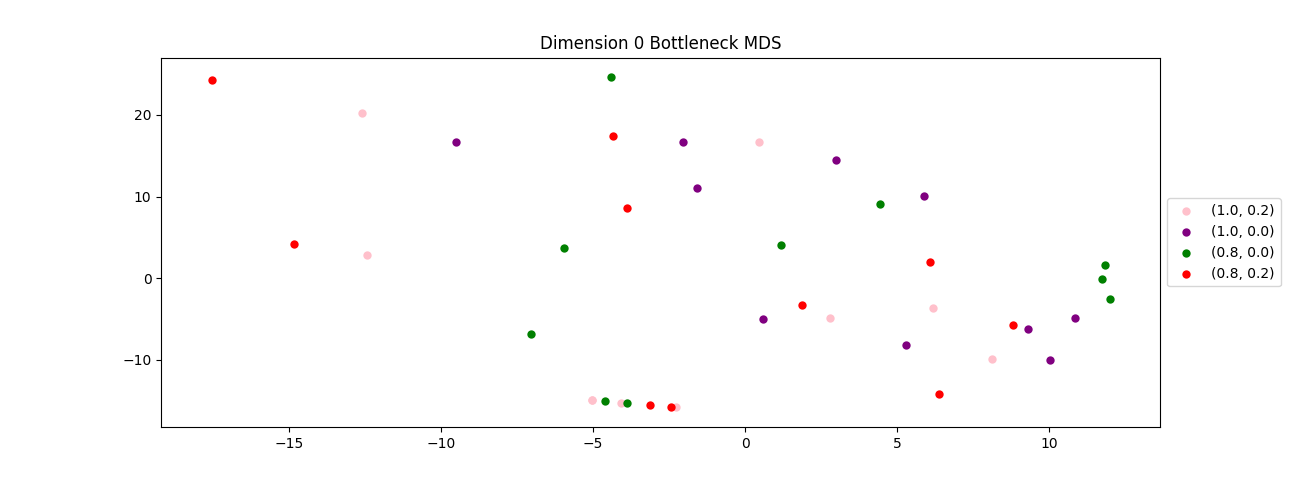
\includegraphics[scale = .5]{dim0mdsripserbott.png}

		\end{subfigure}
		\begin{subfigure}
			\centering
			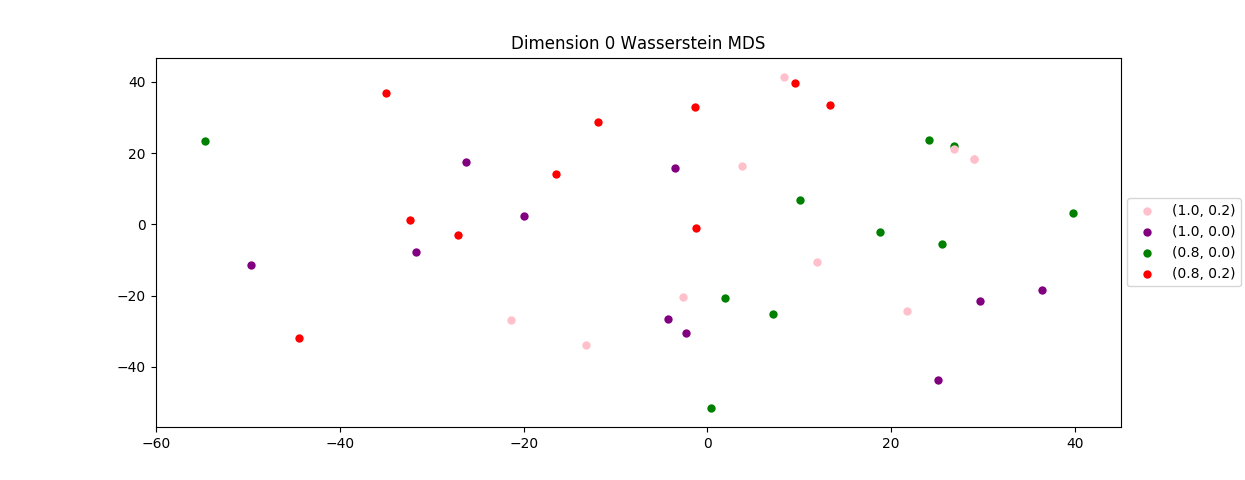
\includegraphics[scale = .5]{dim0mdsripserwasser.png}
		\end{subfigure}
		\caption{Dimension 0 Persistence Diagram MDS Clustering}
	\end{figure*}
	\begin{figure*}[ht!]
		\centering
		\begin{subfigure}
			\centering
			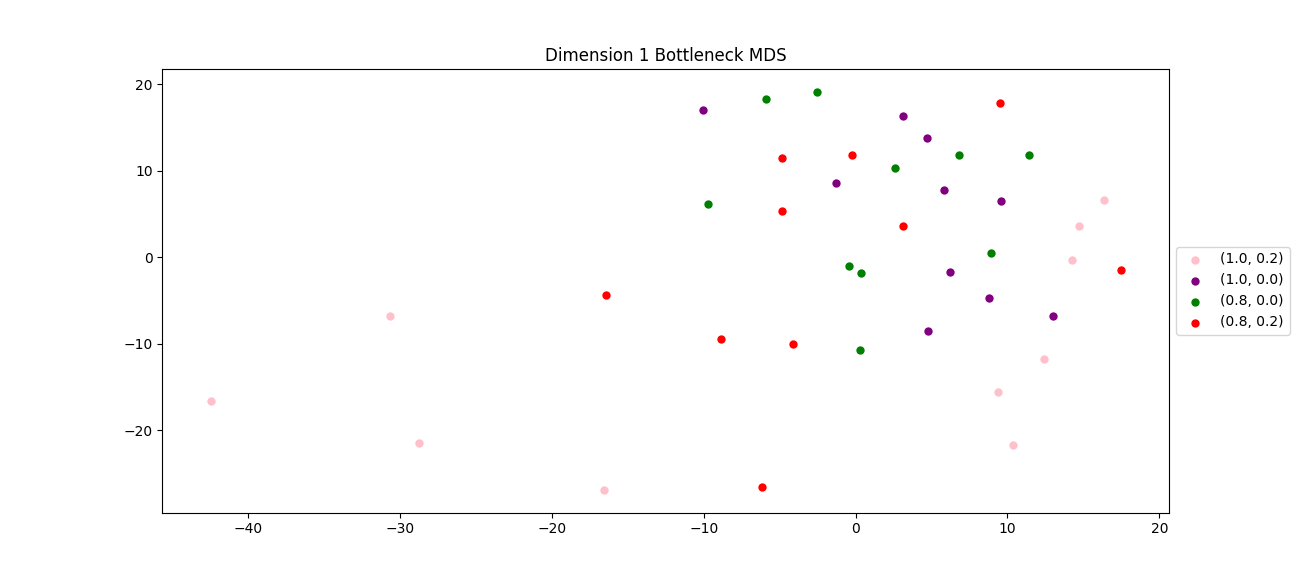
\includegraphics[scale = .5]{dim1mdsripserbott.png}
		\end{subfigure}
		\begin{subfigure}
			\centering
			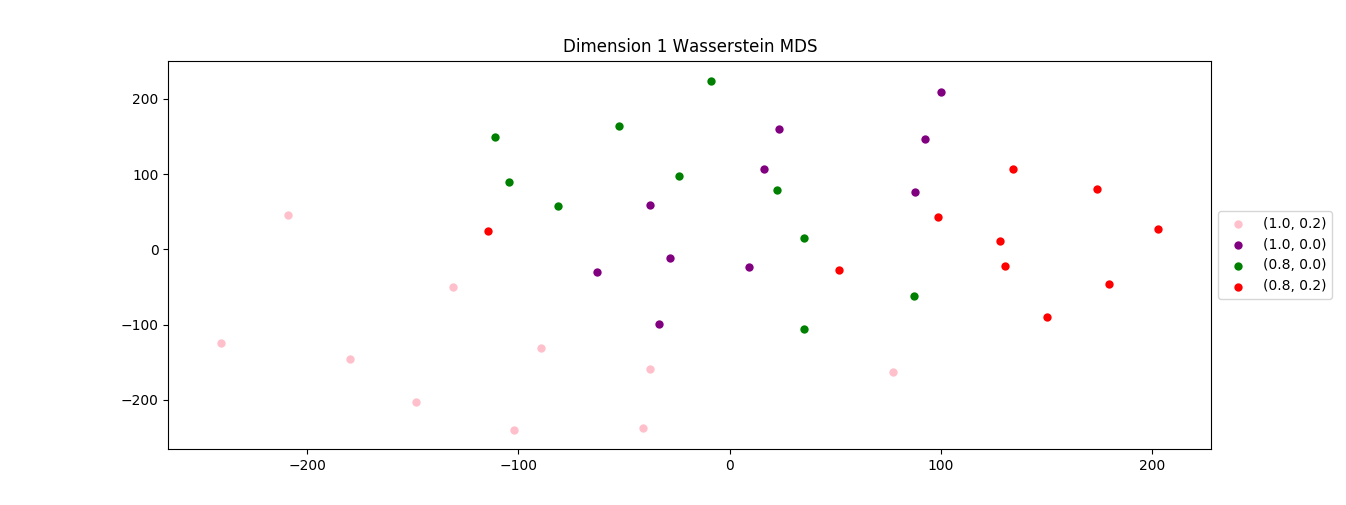
\includegraphics[scale = .5]{dim1mdsripserwasser.png}
		\end{subfigure}
		\caption{Dimension 1 Persistence Diagram MDS Clustering}
	\end{figure*}

	In comparison to these, consider Figure 3 below. It shows the MDS using both Bottleneck and Wasserstein distances for the critical diagrams, using a threshold $\epsilon^2 = 100$.
	\begin{figure*}[ht!]
		\centering
		\begin{subfigure}
			\centering
			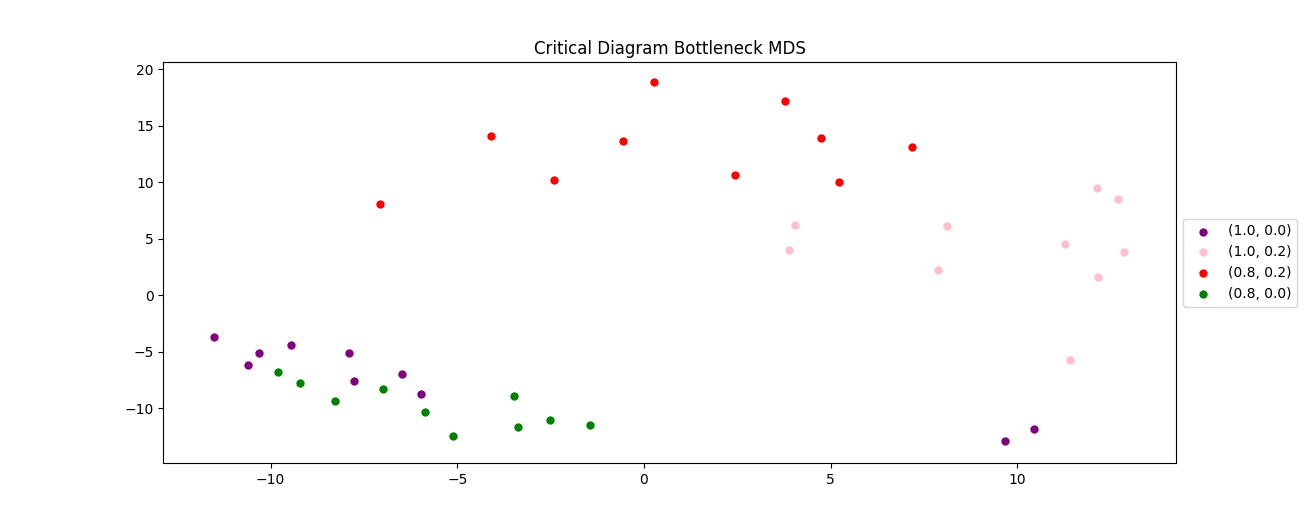
\includegraphics[scale = .5]{mdscritbott.png}
		\end{subfigure}
		\begin{subfigure}
			\centering
			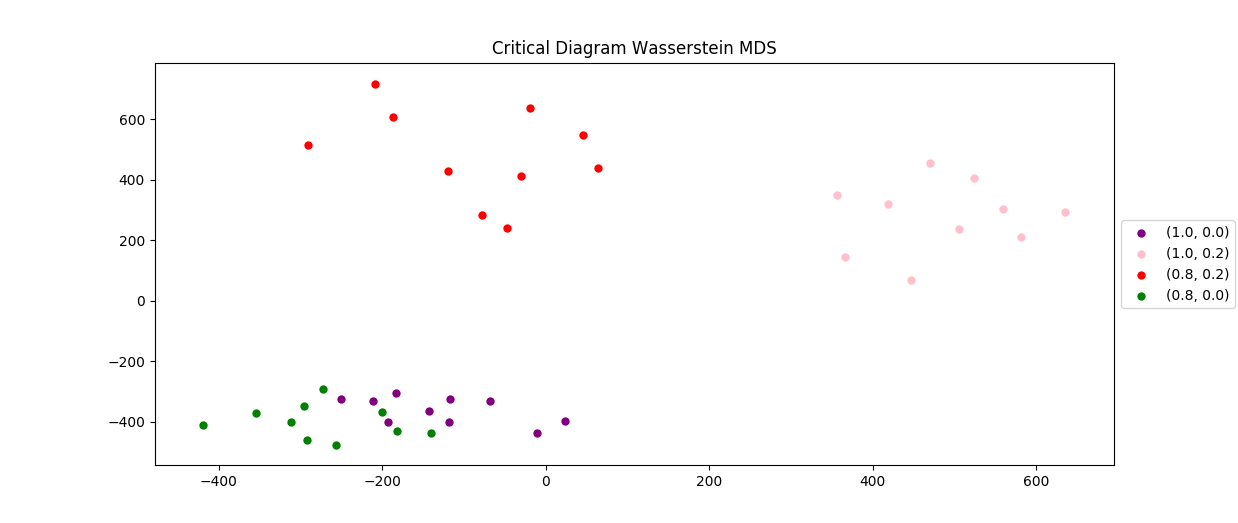
\includegraphics[scale = .5]{mdscritwasser.png}
		\end{subfigure}
		\caption{Critical Diagram MDS Clustering, $\epsilon^2 = 100$}
	\end{figure*}
	From Figure 3 we see much better clustering going on, especially with the Wasserstein metric. This suggests that critical diagrams may have more predictive power in classification than persistent homology for this specific dataset.
	
	\subsection*{\normalfont Machine Learning}
	Using the Persistence Scale Space Kernel (PSSK) with the Support Vector Machine (SVM) and a threshold $\epsilon^2 = 100$ on the critical diagrams, we have Tables 1 and 2.
	\begin{table}[h!]
		\centering
		\begin{tabular}{ |l|c|c|c|c|c|c| } 
			\hline
			Number of Classes & \multicolumn{3}{|c|}{2} & \multicolumn{3}{|c|}{4} \\
			\hline
			Number Training Examples:& 4 & 6 & 8 & 4 & 6 & 8 \\ 
			\hline
			Training Error  & 0.00 & 0.00 & 0.00 & 0.00 & 0.00 & 0.00 \\ 
			\hline
			Testing Error  & 0.50 & 0.25 & 0.75 & 0.5833 & 0.4375 & 0.625\\ 
			\hline
		\end{tabular}
		\caption{Prediction Errors Using Persistence Diagrams, PSSK}
	\end{table}
	\begin{table}[h!]
		\centering
		\begin{tabular}{ |l|c|c|c|c|c|c| } 
			\hline
			Number of Classes & \multicolumn{3}{|c|}{2} & \multicolumn{3}{|c|}{4} \\
			\hline
			Number Training Examples:& 4 & 6 & 8 & 4 & 6 & 8 \\ 
			\hline
			Training Error  & 0.00 & 0.00 & 0.00 & 0.00 & 0.00 & 0.00 \\ 
			\hline
			Testing Error  & 0.00 & 0.00 & 0.00 & 0.0833 & 0.00 & 0.00 \\ 
			\hline
		\end{tabular}
		\caption{Prediction Errors Using Critical Diagrams, PSSK}
	\end{table}
	From this it is clear that using critical diagrams was a much better predictor of mixing specie than persistence diagrams for the PSSK. The persistence diagrams yielded a testing error of, at best, $43.75\%$ whereas the critical diagrams yielded a testing error of, at worst, $8.\bar{3}\%$. 
	
	Continuing, we now look at the results for Persistence Images (PI) again using the SVM. The tables below show prediction errors for various kernels, number of training classes, and number of examples. For brevity, we set the bandwidth hyper-parameter to 0.9 for both persistence and critical diagrams. Again we also use $\epsilon^2 = 100$. When running the program, classification results for different bandwidths are shown.
	
	\begin{table}[h!]
		\centering
		\begin{tabular}{ |l|c|c|c|c|c|c| } 
			\hline
			Number of Classes & \multicolumn{3}{|c|}{2} & \multicolumn{3}{|c|}{4} \\
			\hline
			Number Training Examples:& 4 & 6 & 8 & 4 & 6 & 8 \\ 
			\hline
			RBF Kernel Training Error  & 0.125 & 0.00 & 0.125 & 0.125 & 0.20833 & 0.28125 \\ 
			\hline
			RBF Kernel Testing Error  & 0.25 & 0.125 & 0.25 & 0.50 & 0.4375 & 0.50\\ 
			\hline
			Linear Kernel Training Error  & 0.00 & 0.00 & 0.00 & 0.00 & 0.00 & 0.00 \\ 
			\hline
			Linear Kernel Testing Error  & 0.166 & 0.25 & 0.25 & 0.5833 & 0.50 & 0.625\\ 
			\hline
			Cubic Kernel Training Error  & 0.25 & 0.25 & 0.25 & 0.4375 & 0.54167 & 0.40625 \\ 
			\hline
			Cubic Kernel Testing Error  & 0.333 & 0.125 & 0.50 & 0.70833 & 0.5625 & 0.75\\ 
			\hline
			Sigmoid Kernel Training Error  & 0.125 & 0.00 & 0.125 & 0.1875 & 0.20833 & 0.3125 \\ 
			\hline
			Sigmoid Kernel Testing Error  & 0.25 & 0.125 & 0.25 & 0.50 & 0.4375 & 0.50\\ 
			\hline
		\end{tabular}
		\caption{Prediction Errors Using Persistence Diagrams, PI}
	\end{table}
	\begin{table}[h!]
		\centering
		\begin{tabular}{ |l|c|c|c|c|c|c| } 
			\hline
			Number of Classes & \multicolumn{3}{|c|}{2} & \multicolumn{3}{|c|}{4} \\
			\hline
			Number Training Examples:& 4 & 6 & 8 & 4 & 6 & 8 \\ 
			\hline
			RBF Kernel Training Error  & 0.375 & 0.4166 & 0.375 & 0.00 & 0.166 & 0.1875 \\ 
			\hline
			RBF Kernel Testing Error  & 0.4167 & 0.375 & 0.50 & 0.125 & 0.25 & 0.25\\ 
			\hline
			Linear Kernel Training Error  & 0.00 & 0.00 & 0.00 & 0.00 & 0.00 & 0.00 \\ 
			\hline
			Linear Kernel Testing Error  & 0.0833 & 0.00 & 0.00 & 0.125 & 0.00 & 0.00\\ 
			\hline
			Cubic Kernel Training Error  & 0.25 & 0.167 & 0.25 & 0.00 & 0.166 & 0.15625 \\ 
			\hline
			Cubic Kernel Testing Error  & 0.333 & 0.25 & 0.25 & 0.125 & 0.25 & 0.125\\ 
			\hline
			Sigmoid Kernel Training Error  & 0.375 & 0.4166 & 0.00 & 0.1875 & 0.166 & 0.1875 \\ 
			\hline
			Sigmoid Kernel Testing Error  & 0.4167 & 0.375 & 0.50 & 0.125 & 0.25 & 0.25\\ 
			\hline
		\end{tabular}
		\caption{Prediction Errors Using Critical Diagrams, PI}
	\end{table}
	From these tables we notice a few curious details. The first is that for a smaller number of classes used for classification, the persistence diagrams outperform the critical diagrams but the converse was true for a larger number of classes used for classification. However, this was not the case for the linear kernel. With this kernel, prediction using critical diagrams had a worst predictive error of $12.5\%$ whereas the best predictive error using persistence diagrams was $16.5\%$. 

\section*{\normalfont Evaluation}
Overall the critical diagrams served as good features for classifying mixing specie. Though persistence diagrams proved to be more effective informers than critical diagrams on a few kernels, critical diagrams almost always provided more effective information for the machine learning classifiers. The error in training and testing was surprisingly low on many of the kernels, and we conclude that critical diagrams are a source of sufficient information to differentiate RTIs formed by varying liquid densities.

\section*{\normalfont Deliverables} As stated before, our RTI simulations were generated by the package at \url{http://www.palabos.org}, and we provide those, as well as a script to generate them. The boundary extraction algorithm was written by ourselves in Java, and we provide the source code, as well as the boundary images and point clouds associated with the simulations provided. Finally, we also wrote a python script that sent the point clouds through the machine learning pipeline, and we provide the source code for that as well.

\section*{\normalfont Conclusions and Discussions}
	We analyzed Rayleigh-Taylor Instabilities by using simulations and sampling points from their isosurfaces. The project objective was to classify RTIs by the densities of the fluids involved, and we did this by examining two topological features: persistent homology, and critical point graphs, both represented as persistent/critical diagrams. This demonstrates that despite the complicated nature of fluid dynamics, there are features in RTIs that can be used to reliably categorize them into similar classes. Nevertheless, one insight from our findings is that features that show promise in several areas may not always be sufficient in describing the nature of RTIs. From here, research could expand these techniques to a more general, three dimensional setting. The paper that inspired our work does that to some extent, but only analyzing bubble maxima evolution and Morse-Smale complexes.
\bibliography{mybib}{}
\bibliographystyle{plain}

\end{document}
